\documentclass[twocolumn]{article}
\usepackage{graphicx}
\usepackage{amsmath}

\usepackage[backend=bibtex]{biblatex}
\addbibresource{refs.bib}


\title{GLOBAL ILLUMINATION USING MONTE CARLO PATH TRACING \\ {\small\vspace{-1.0em} ADVANCED GLOBAL ILLUMINATION AND RENDERING, TNCG15}}

\author{Isabelle Forsman\\isafo268@student.liu.se}
\date{\today}

\begin{document}
\maketitle

\begin{abstract}

\end{abstract}


\section{Introduction}
Local lighting models only takes the direct illumination into account. In order to render photo realistic images both direct illumination and indirect illumination are needed and thus the local lighting model does not suffice. Global illumination algorithms account for both direct and indirect illumination and can be used to render photo realistic images. Global illumination models are however computationally heavy and require more time to render. There exist several global illumination algorithms and there has been much research in the area in order to improve the performance and result.

\subsection{Monte Carlo ray tracing}
Monte Carlo path tracing is a method where rays are traced from the camera out in the scene in order to determine how much light enters each pixel on the image plane \cite{CG:PP}. Since it is not possible to calculate the incoming light from all directions for all points in the scene a new ray is generated using Monte Carlo integration to produce uniformly distributed random samples over a hemisphere. Monte Carlo path tracing is a computationally heavy algorithm and rendering time is dependent on the complexity of the scene.

Monte Carlo ray tracing is usually divided into two categories: Distribution ray tracing and path tracing \cite{hq}. Distribution ray tracing shoots multiple rays from each surface intersection point in order to sample the incoming light over the hemisphere. Thus this method usually produce a great number of rays after a few number of reflections. In order to reduce the number of rays the number of rays reflected are reduced after the ray has been reflected a few levels. Path tracing on the other hand only shots one ray per surface intersection point. Instead multiple rays are shot through each pixel. This avoids the explosion of the number of rays but it is harder to ensure that the rays are reflected with a good distribution. Path tracing allows camera effects like depth-of-field and motion blur to be implemented efficiently.

\subsection{Photon mapping}
Photon mapping is a method used together with Monte Carlo path tracing in order to reduce the number of calculations needed and thus improve rendering times. The photon mapping algorithm is a two pass rendering method \cite{jensen}. During the first pass photons are emitted from the light sources in the scene. A photon map is built up containing information about where in the scene the emitted photons ended up. During the second pass the photon map is used to estimate the radiance. The use of shadow photons also allows the number of shadow rays used in the Monte Carlo path tracing to be reduced.

\subsection{Radiosity}
The radiosity method differs from the previously mentioned methods in that it considers where the energy emitted by the light sources end up and records it \cite{CG:PP}. This is done by partitioning all surfaces in the scene into small patches. Then by considering how each patch send and receive light energy the global diffuse inter-object reflection can be approximated. The Radiosity method is limited to lambertian reflectors but the method can be used in real time for dynamically changing scenes \cite{Rfb}.

\subsection{Structure of the paper}

\section{Background}

\subsection{The rendering equation}

The light contribution from a point in the scene is made up of how much light is emitted from the object in the direction of the camera and how much incoming light is reflected towards the camera. This is calculated using the rendering equation \ref{eq:rendereq}.

\begin{align}
\label{eq:rendereq}
\begin{split}
	 L(\mathbf{x} \rightarrow \omega_{out}) = L_e(\mathbf{x} \rightarrow \omega_{out}) + \\ \int_{\Omega} f_r(\mathbf{x}, \omega_{in}, \omega_{out})L(\mathbf{x} \leftarrow \omega_{in})cos\theta_{in}d\omega_{in}
\end{split}
\end{align}

The first part of the rendering equation $L_e(\mathbf{x} \rightarrow \omega_{out})$ is the light emitted form the point $\mathbf{x}$ in the direction $\omega_{out}$. The integral part of the equations is the incoming light that is reflected into the  direction $\omega_{out}$ integrated over the hemisphere $\Omega$, see fig. \ref{fig:hemisphere}.

\begin{figure}[ht]
\centering
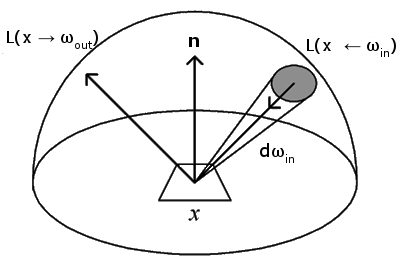
\includegraphics[width=1.0\linewidth]{pics/hemisphere.png}
\caption{\label{fig:hemisphere} }
\end{figure}

The individual terms of the integral part are:

\vspace*{1em}

$f_r(\mathbf{x}, \omega_{in}, \omega_{out})$, is the Bidirectional reflectance distribution function or for short the BRDF. This term describes how much of the incoming light from the considered point on the hemisphere is reflected in the viewing direction. %mention different brdfs?

\vspace*{1em}

$L(\mathbf{x} \leftarrow \omega_{in})$, describes ho much light is coming in from the considered point on the hemisphere.

\vspace*{1em}

$cos\theta_{in}$, describes the area that the incoming light from the considered point on the hemisphere is distributed on. As the incoming light gets more perpendicular to the surface normal the light is distributed on a larger area and less is reflected.

\subsection{Reflection models}
There are numerous reflection models that can be used in ray tracing to represent the reflection of different materials. A common reflection model for diffuse reflections is the Lambert's cosine law. The Lambert's cosine law declares that the light that is reflected of off a surface is proportional to the cosine of the angle between the surface normal and the incoming light. A Lambertian reflector has the BRDF of $\frac{\rho}{\pi}$ where $\rho$ is the albedo, the reflection coefficient, of the surface.
Another reflection model for diffuse reflections from rough surfaces is the Oren-Nayar reflection model. The Oren-Nayar reflection model assumes the surface consists of symmetric cavities creating a rough surface. The roughness of the surface is produced using a probability function, usually the Gaussian distribution. The Oren-Nayar reflection model assumes that the object is a Lambertian reflector.
Common reflection models for computing the highlights on glossy and specular objects are the Phong cosine-power formula or the Ward's isotropic and anisotropic reflection models \cite{hq}. These are however beyond the scope of this paper.

\subsection{Monte Carlo integration}
	Since it is not possible to calculate the incoming radiance for an infinite number of infinitesimal $d\omega$ a set of random sample points are used instead. Monte Carlo integration estimates a numerical integration using random numbers. The random points used are placed where the integrand is evaluated. 

For lambertian reflectors the randomly produced directions should be uniformly sampled over the hemisphere. The density $\rho$ for a hemisphere is $\rho = \frac{1}{2\pi}$ \cite{CG:PP}. Producing the random direction is the done by:


\begin{align*}
	\begin{split}
		\theta = 2\pi u \\
		\phi = cos^{-1}(2v - 1)
	\end{split}
\end{align*}

where $u$ and $v$ are randomly generated values within the distribution $[0, 1]$.

\subsection{Ray surface intersection}
In order to determine what objects and where on the object a ray hits we need to calculate its intersection between all objects in the scene. In case of multiple intersections the nearest one is used. A ray is in this case a semi-infinite line defined by an origin $\mathbf{o}$ and a direction $\mathbf{d}$ and every point on the ray is given by:

\begin{equation}
	\label{eq:ray}
	\mathbf{x}(t) = \mathbf{o} + t\mathbf{d}
\end{equation}

for $t \geq 0$. This section provides an overview of ray-object intersection calculations for triangles and implicit spheres. 

\subsubsection{Ray-triangle intersection}
Any point on a triangle can be expressed using eq. \ref{eq:bc} where $u$, $v$ and $ w = 1 - u - v$ are the barycentric coordinates \cite{hq}. If the condition $u$, $v$, $w \leq 1$ is satisfied the point lies on the triangle. Assuming that the ray intersects the triangle by setting the expression of the ray, eq. \ref{eq:ray},s equal to a point on the triangle and simplifying the expression one receives eq. \ref{eq:simp}. Using Cramer's rule the three unknown variables can be solved for resulting in eq. \ref{eq:triInt}, where $E_1 = \mathbf{v}_1 - \mathbf{v}_0$ and $E_2 = \mathbf{v}_2 - \mathbf{v}_0$, $T = o - \mathbf{v}_0$, $P = D \times E_2$, $Q = T \times E_1$ and D is the normalized direction of the ray.

\begin{equation}
	\label{eq:bc}	
	T(u,v) = (1 - u - v)\mathbf{v}_0 + u\mathbf{v}_1 + v\mathbf{v}_2
\end{equation}

\begin{equation}
	\label{eq:simp}
	u(\mathbf{v}_1 - \mathbf{v}_0) + v(\mathbf{v}_2 - \mathbf{v}_0) - t\mathbf{d} = \mathbf{p} - \mathbf{v}_0
\end{equation}

\begin{equation}
\label{eq:triInt}
\begin{pmatrix}
	t \\
  	u \\
  	v 
\end{pmatrix}
= \frac{1}{\mathbf{P} \cdot \mathbf{E}_1}
\begin{pmatrix}
	  	\mathbf{Q} \cdot \mathbf{E}_2 \\
  		\mathbf{P} \cdot \mathbf{T} \\
  		\mathbf{Q} \cdot \mathbf{D}
\end{pmatrix}
\end{equation}

\subsubsection{Ray-sphere intersection}
A point $\mathbf{x}$ is on the surface of a sphere with radius $r$ and origin $c$ if it satisfies eq. \ref{eq:sphereC} \cite{hq}. Thus the intersections between the ray and sphere surface satisfy this condition. Using eq. \ref{eq:ray} to express the ray and solving for d results in eq. \ref{eq:sphereInt}, where $b = 2\mathbf{d} \cdot (\mathbf{o} \cdot \mathbf{c})$, $a = \mathbf{d} \cdot \mathbf{d}$ and $c = (\mathbf{o} - \mathbf{c}) \cdot (\mathbf{o} - \mathbf{c}) - r^2$

\begin{equation}
	\label{eq:sphereC}
	||\mathbf{x} - \mathbf{o}||^2 = r^2
\end{equation}

\begin{equation}
	\label{eq:sphereInt}
	t = - \frac{b}{2} \pm \sqrt{\frac{b}{2}^2 - ac}
\end{equation}

\subsection{Direct illumination}
Direct illumination is approximated by sending out a ray from the intersection point of an object to the light source. This ray is called a shadow ray and is used to test whether the intersectionpoint on the object is visible to the light source. Since area light sources are used every point on the light source would have to be tested for visibility. This is not practical and thus a set of random points on the area light source are tested. These random points are generated using two random values $u$ and $v$ within the distribution $0 \leq u,v \leq 1$. These random values are regenerated until they satisfy the condition $u + v < 1$ and the point $\mathbf{q}$ can be calculated using barycentric coordinates

\begin{equation*}
	\mathbf{q} = (1 - u - v)\mathbf{v}_0 + u\mathbf{v}_1 + v\mathbf{v}_2
\end{equation*}

where $\mathbf{v}_0, \mathbf{v}_1$ and $\mathbf{v}_2$ are the vertices of the light source triangle. The direct illumination can then be estimated using

%mention the PDE and choise of it some where
\begin{align*}
	L_D(x_N \rightarrow -\omega_{N-1}) = \\
	 \frac{AL_0}{M} \sum_{i=1}^{M}f_r(x_N, \omega_S, i, -\omega_{N-1})V(x_N, q_i)G(x_n, q_i)
\end{align*}

where $M$ is the number of shadow rays, $x_N$ is the intersection point the shadow rays are cast from and $q_i$ are the $M$ randomly generated points on the light source. $V(x_N, q_i)$ is the visibility function and $G(x_n, q_i)$ is the geometric term calculated by 

\begin{equation*}
	G(x_n, q) = \frac{cos\alpha cos\beta}{d^2}
\end{equation*}

where d is the length of the shadow ray.

\subsection{Indirect illumination}

\section{Results}


\newpage
\printbibliography

\end{document}

%\begin{figure*}[ht]
%\centering
%\includegraphics[width=1.0\linewidth]{pics/picture.png}
%\caption{\label{fig:label} }
%\end{figure*}
